\documentclass[a4paper, 12pt]{article} % Статья формата A4, 12 шрифт
\usepackage{fontspec} % Для выбора шрифта
\setmainfont{Times New Roman} % Устанавливаем шрифт Times New Roman
\usepackage[russian]{babel} % Поддержка русского языка
\usepackage{amsmath} % Пакет для математических формул (\dfrac, cases)
\usepackage{caption} % Пакет для настройки подписей (\caption*)
\usepackage{graphicx} % Для вставки картинок (\includegraphics)
\usepackage{geometry} % Пакет для настройки размера страницы и полей документа
\geometry{top=2cm, bottom=2cm, left=2cm, right=2cm} % Настройка полей

\begin{document}
	\textbf{2.7.}
	Даны значения вещественных переменных \( x \) и \( y \). Вычислить значение \( z \), пользуясь
	функцией вида \( \text{ABS}(w) \) для определения модуля \( w \) при вещественном аргументе \( w \)
	и исходя из следующего правила вычисления \( z \):
	% \text - для напечатания обычного текста, а не математической формулы
	\[ % Для вставки формул отдельной строкой по центру
	z =
	\begin{cases} % фигурные скобки для системы уравнений
		\dfrac{|x| + |y|}{2}, & \text{при } x < y; \\
		1 + 2|x|, & \text{при } x \geq y. % greater or equal (>=)
	\end{cases}
	\]
	
	\begin{figure}[h] % here (размещаем рисунок именно здесь)
		\centering % Выравнивание по центру
		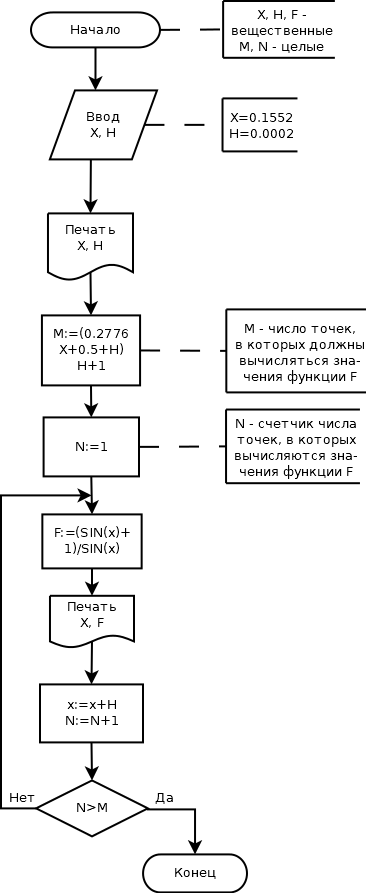
\includegraphics[width=0.4\textwidth]{Блок-схема.png}
		\caption*{Рис. 11} % Отключение автоматической подписи рисунков
	\end{figure}
\end{document}